\documentclass{standalone}
\usepackage{tikz}
\usetikzlibrary{patterns, positioning}

\begin{document}
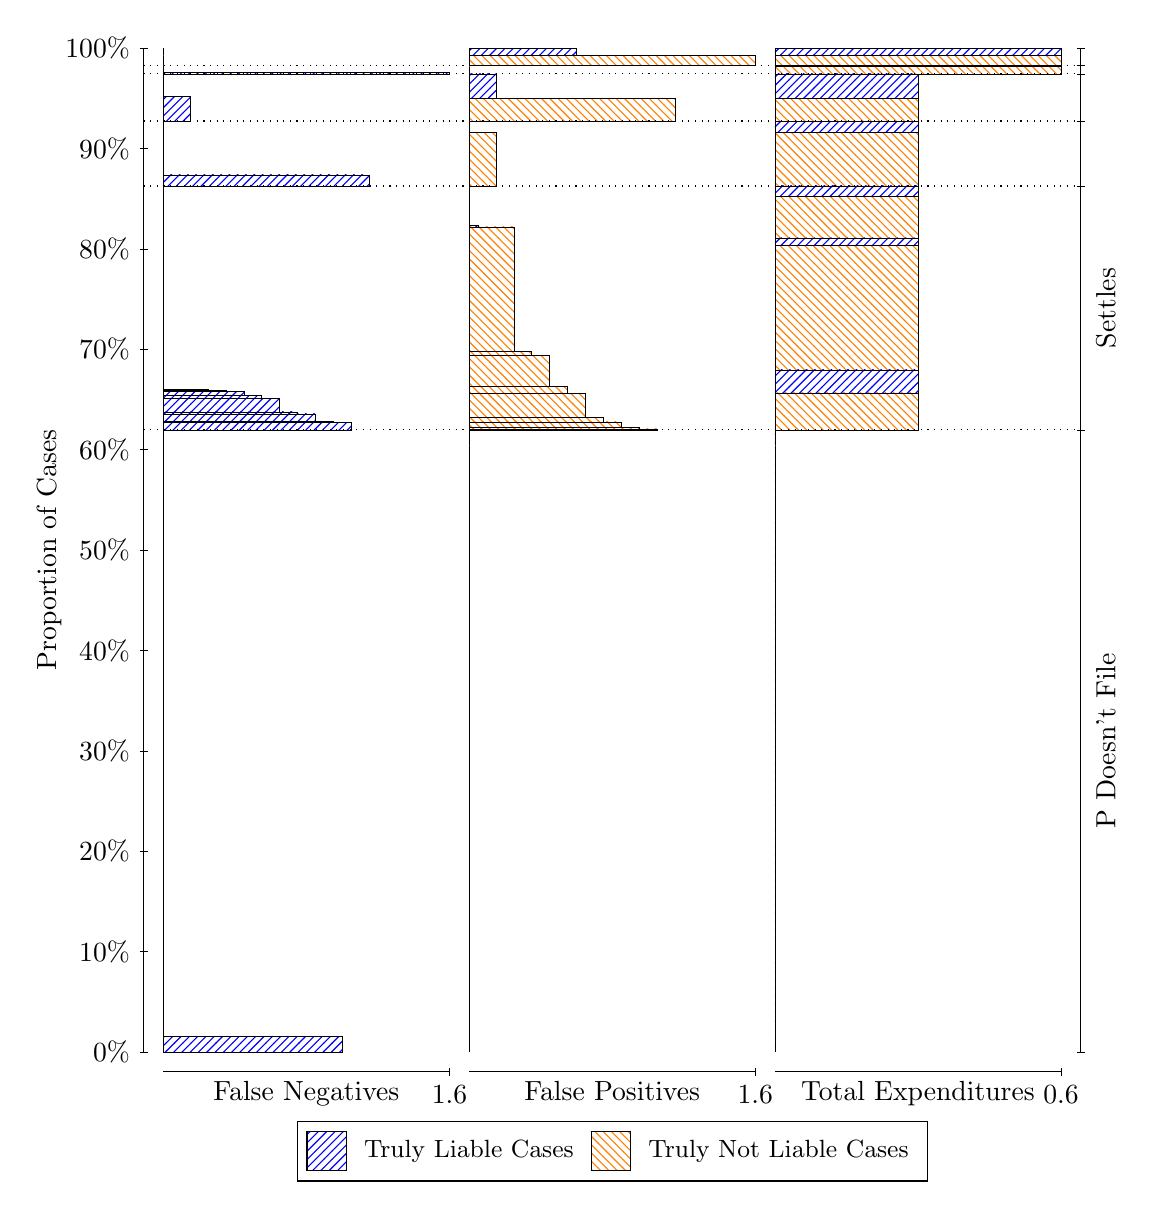
\begin{tikzpicture}
\draw[black, very thin] (1.5,1.75) -- (1.5,14.5);
\node[rotate=90, anchor=center] at (0.3, 8.125) {Proportion of Cases};
\draw[black, very thin] (1.45,1.75) -- (1.55,1.75);
\node[anchor=east] at (1.45, 1.75) {0\%};
\draw[black, very thin] (1.45,3.025) -- (1.55,3.025);
\node[anchor=east] at (1.45, 3.025) {10\%};
\draw[black, very thin] (1.45,4.3) -- (1.55,4.3);
\node[anchor=east] at (1.45, 4.3) {20\%};
\draw[black, very thin] (1.45,5.575) -- (1.55,5.575);
\node[anchor=east] at (1.45, 5.575) {30\%};
\draw[black, very thin] (1.45,6.85) -- (1.55,6.85);
\node[anchor=east] at (1.45, 6.85) {40\%};
\draw[black, very thin] (1.45,8.125) -- (1.55,8.125);
\node[anchor=east] at (1.45, 8.125) {50\%};
\draw[black, very thin] (1.45,9.4) -- (1.55,9.4);
\node[anchor=east] at (1.45, 9.4) {60\%};
\draw[black, very thin] (1.45,10.675) -- (1.55,10.675);
\node[anchor=east] at (1.45, 10.675) {70\%};
\draw[black, very thin] (1.45,11.95) -- (1.55,11.95);
\node[anchor=east] at (1.45, 11.95) {80\%};
\draw[black, very thin] (1.45,13.225) -- (1.55,13.225);
\node[anchor=east] at (1.45, 13.225) {90\%};
\draw[black, very thin] (1.45,14.5) -- (1.55,14.5);
\node[anchor=east] at (1.45, 14.5) {100\%};

\draw[black, very thin] (13.4,1.75) -- (13.4,14.5);
\draw[black, very thin] (13.35,1.75) -- (13.45,1.75);
\node[anchor=west] at (13.35, 1.75) {};
\draw[black, very thin] (13.35,9.6497) -- (13.45,9.6497);
\node[anchor=west] at (13.35, 9.6497) {};
\draw[black, very thin] (13.35,12.748) -- (13.45,12.748);
\node[anchor=west] at (13.35, 12.748) {};
\draw[black, very thin] (13.35,13.573) -- (13.45,13.573);
\node[anchor=west] at (13.35, 13.573) {};
\draw[black, very thin] (13.35,14.172) -- (13.45,14.172);
\node[anchor=west] at (13.35, 14.172) {};
\draw[black, very thin] (13.35,14.281) -- (13.45,14.281);
\node[anchor=west] at (13.35, 14.281) {};
\draw[black, very thin] (13.35,14.5) -- (13.45,14.5);
\node[anchor=west] at (13.35, 14.5) {};

\draw[black, very thin, pattern color=blue, pattern=north east lines] (1.75,1.75) rectangle (4.0208,1.9467);
\draw[black, very thin, pattern color=orange, pattern=north west lines] (1.75,1.9467) rectangle (1.75,9.6497);
\draw[black, very thin, pattern color=blue, pattern=north east lines] (1.75,9.6497) rectangle (4.1344,9.7452);
\draw[black, very thin, pattern color=blue, pattern=north east lines] (1.75,9.7452) rectangle (3.9073,9.7557);
\draw[black, very thin, pattern color=blue, pattern=north east lines] (1.75,9.7557) rectangle (3.6802,9.8545);
\draw[black, very thin, pattern color=blue, pattern=north east lines] (1.75,9.8545) rectangle (3.4531,9.8779);
\draw[black, very thin, pattern color=blue, pattern=north east lines] (1.75,9.8779) rectangle (3.226,10.047);
\draw[black, very thin, pattern color=blue, pattern=north east lines] (1.75,10.047) rectangle (2.999,10.084);
\draw[black, very thin, pattern color=blue, pattern=north east lines] (1.75,10.084) rectangle (2.7719,10.136);
\draw[black, very thin, pattern color=blue, pattern=north east lines] (1.75,10.136) rectangle (2.5448,10.152);
\draw[black, very thin, pattern color=blue, pattern=north east lines] (1.75,10.152) rectangle (2.3177,10.169);
\draw[black, very thin, pattern color=orange, pattern=north west lines] (1.75,10.169) rectangle (1.75,12.748);
\draw[black, very thin, pattern color=blue, pattern=north east lines] (1.75,12.748) rectangle (4.3615,12.89);
\draw[black, very thin, pattern color=orange, pattern=north west lines] (1.75,12.89) rectangle (1.75,13.573);
\draw[black, very thin, pattern color=blue, pattern=north east lines] (1.75,13.573) rectangle (2.0906,13.882);
\draw[black, very thin, pattern color=orange, pattern=north west lines] (1.75,13.882) rectangle (1.75,14.172);
\draw[black, very thin, pattern color=blue, pattern=north east lines] (1.75,14.172) rectangle (5.3833,14.186);
\draw[black, very thin, pattern color=orange, pattern=north west lines] (1.75,14.186) rectangle (1.75,14.281);
\draw[black, very thin, pattern color=orange, pattern=north west lines] (1.75,14.281) rectangle (1.75,14.406);
\draw[black, very thin, pattern color=blue, pattern=north east lines] (1.75,14.406) rectangle (1.75,14.5);
\draw[black, very thin, pattern color=orange, pattern=north west lines] (5.6333,1.75) rectangle (5.6333,9.453);
\draw[black, very thin, pattern color=blue, pattern=north east lines] (5.6333,9.453) rectangle (5.6333,9.6497);
\draw[black, very thin, pattern color=orange, pattern=north west lines] (5.6333,9.6497) rectangle (8.0177,9.6644);
\draw[black, very thin, pattern color=orange, pattern=north west lines] (5.6333,9.6644) rectangle (7.7906,9.6833);
\draw[black, very thin, pattern color=orange, pattern=north west lines] (5.6333,9.6833) rectangle (7.5635,9.7507);
\draw[black, very thin, pattern color=orange, pattern=north west lines] (5.6333,9.7507) rectangle (7.3365,9.8083);
\draw[black, very thin, pattern color=orange, pattern=north west lines] (5.6333,9.8083) rectangle (7.1094,10.118);
\draw[black, very thin, pattern color=orange, pattern=north west lines] (5.6333,10.118) rectangle (6.8823,10.121);
\draw[black, very thin, pattern color=orange, pattern=north west lines] (5.6333,10.121) rectangle (6.8823,10.201);
\draw[black, very thin, pattern color=orange, pattern=north west lines] (5.6333,10.201) rectangle (6.6552,10.6);
\draw[black, very thin, pattern color=orange, pattern=north west lines] (5.6333,10.6) rectangle (6.4281,10.647);
\draw[black, very thin, pattern color=orange, pattern=north west lines] (5.6333,10.647) rectangle (6.201,12.228);
\draw[black, very thin, pattern color=blue, pattern=north east lines] (5.6333,12.228) rectangle (5.7469,12.245);
\draw[black, very thin, pattern color=blue, pattern=north east lines] (5.6333,12.245) rectangle (5.6333,12.748);
\draw[black, very thin, pattern color=orange, pattern=north west lines] (5.6333,12.748) rectangle (5.974,13.43);
\draw[black, very thin, pattern color=blue, pattern=north east lines] (5.6333,13.43) rectangle (5.6333,13.573);
\draw[black, very thin, pattern color=orange, pattern=north west lines] (5.6333,13.573) rectangle (8.2448,13.863);
\draw[black, very thin, pattern color=blue, pattern=north east lines] (5.6333,13.863) rectangle (5.974,14.172);
\draw[black, very thin, pattern color=orange, pattern=north west lines] (5.6333,14.172) rectangle (5.6333,14.267);
\draw[black, very thin, pattern color=blue, pattern=north east lines] (5.6333,14.267) rectangle (5.6333,14.281);
\draw[black, very thin, pattern color=orange, pattern=north west lines] (5.6333,14.281) rectangle (9.2667,14.406);
\draw[black, very thin, pattern color=blue, pattern=north east lines] (5.6333,14.406) rectangle (6.9958,14.5);
\draw[black, very thin, pattern color=orange, pattern=north west lines] (9.5167,1.75) rectangle (9.5167,9.453);
\draw[black, very thin, pattern color=blue, pattern=north east lines] (9.5167,9.453) rectangle (9.5167,9.6497);
\draw[black, very thin, pattern color=orange, pattern=north west lines] (9.5167,9.6497) rectangle (11.333,10.121);
\draw[black, very thin, pattern color=blue, pattern=north east lines] (9.5167,10.121) rectangle (11.333,10.412);
\draw[black, very thin, pattern color=orange, pattern=north west lines] (9.5167,10.412) rectangle (11.333,11.994);
\draw[black, very thin, pattern color=blue, pattern=north east lines] (9.5167,11.994) rectangle (11.333,12.09);
\draw[black, very thin, pattern color=orange, pattern=north west lines] (9.5167,12.09) rectangle (11.333,12.616);
\draw[black, very thin, pattern color=blue, pattern=north east lines] (9.5167,12.616) rectangle (11.333,12.748);
\draw[black, very thin, pattern color=orange, pattern=north west lines] (9.5167,12.748) rectangle (11.333,13.43);
\draw[black, very thin, pattern color=blue, pattern=north east lines] (9.5167,13.43) rectangle (11.333,13.573);
\draw[black, very thin, pattern color=orange, pattern=north west lines] (9.5167,13.573) rectangle (11.333,13.863);
\draw[black, very thin, pattern color=blue, pattern=north east lines] (9.5167,13.863) rectangle (11.333,14.172);
\draw[black, very thin, pattern color=orange, pattern=north west lines] (9.5167,14.172) rectangle (13.15,14.267);
\draw[black, very thin, pattern color=blue, pattern=north east lines] (9.5167,14.267) rectangle (13.15,14.281);
\draw[black, very thin, pattern color=orange, pattern=north west lines] (9.5167,14.281) rectangle (13.15,14.406);
\draw[black, very thin, pattern color=blue, pattern=north east lines] (9.5167,14.406) rectangle (13.15,14.5);
\draw[black, dotted] (1.5,9.6497) -- (13.4,9.6497);
\draw[black, dotted] (1.5,12.748) -- (13.4,12.748);
\draw[black, dotted] (1.5,13.573) -- (13.4,13.573);
\draw[black, dotted] (1.5,14.172) -- (13.4,14.172);
\draw[black, dotted] (1.5,14.281) -- (13.4,14.281);
\draw[black, very thin] (1.75,1.5) -- (5.3833,1.5);
\node[anchor=north] at (3.5667, 1.5) {False Negatives};
\draw[black, very thin] (5.3833,1.45) -- (5.3833,1.55);
\node[anchor=north] at (5.3833, 1.45) {1.6};

\draw[black, very thin] (5.6333,1.5) -- (9.2667,1.5);
\node[anchor=north] at (7.45, 1.5) {False Positives};
\draw[black, very thin] (9.2667,1.45) -- (9.2667,1.55);
\node[anchor=north] at (9.2667, 1.45) {1.6};

\draw[black, very thin] (9.5167,1.5) -- (13.15,1.5);
\node[anchor=north] at (11.333, 1.5) {Total Expenditures};
\draw[black, very thin] (13.15,1.45) -- (13.15,1.55);
\node[anchor=north] at (13.15, 1.45) {0.6};

\node[black, centered, rotate=90] at (13.72, 5.6998) {P Doesn't File};
\node[black, centered, rotate=90] at (13.72, 11.199) {Settles};





\draw (7.449999999999999,1.5) node[draw=none] (baseCoordinate) {};
\begin{scope}[align=center]
        \matrix[scale=0.5, draw=black, below=0.5cm of baseCoordinate, nodes={draw}, column sep=0.1cm]{
            \node[rectangle, draw, minimum width=0.5cm, minimum height=0.5cm, pattern=north east lines, pattern color=blue] {}; &
            \node[draw=none, font=\small] (B) {Truly Liable Cases}; &
            \node[rectangle, draw, minimum width=0.5cm, minimum height=0.5cm, pattern=north west lines, pattern color=orange] {}; &
            \node[draw=none, font=\small] (B) {Truly Not Liable Cases}; \\
            };
\end{scope}

\end{tikzpicture}
\end{document}